%%%%%%%%%%%%%%%%%%%%%%%%%%%%%%%%%%%%%%%%%%%%%%%%%%%%%%%%%%%%%%%%%%%%%%%%%%%%%%%%
\subsection{Μεθοδολογία αξιολόγησης, περιβάλλοντα, και συμβολισμοί}
\label{subsection:02_01_03:01}

Η αξιολόγηση όλων των συνδυασμών των μεθόδων χάραξης μονοπατιών και ελεγκτών
κίνησης που εξετάζονται στην παρούσα διατριβή πραγματοποιείται σε προσομοιωμένα
και πραγματικά περιβάλλοντα. Το ρομπότ που χρησιμοποιήθηκε σε όλες τις συνθήκες
είναι η δεύτερη έκδοση του
Turtlebot,\footnote{\url{https://www.turtlebot.com/turtlebot2/}} ένα ρομπότ με
διαφορική κίνηση και κυκλικό αποτύπωμα ακτίνας $r=0.175$ m. Τα δύο
προσομοιωμένα περιβάλλοντα στα οποία έγινε συγκριτική αξιολόγηση όλων των
αλγορίθμων είναι διαθέσιμοι κόσμοι του περιβάλλοντος προσομοίωσης
Gazebo.\footnote{\url{http://gazebosim.org/}} Αυτοί οι κόσμοι προσομοιώνουν με
ακρίβεια τις περισσότερες από τις συνθήκες που θα αντιμετώπιζε μια επίγεια
κινητή βάση σε ένα στατικό περιβάλλον εσωτερικού χώρου: διαδρόμους διαφορετικού
πλάτους, στενά περάσματα όπου η ικανοποίηση των περιορισμών είναι κρίσιμη και
ευκολότερα παραβιάσιμη ενώ δοκιμάζουν την ικανότητα των ελεγκτών κίνησης να
εκτελούν λεπτές κινήσεις, αναστροφές, πολλαπλές διαδοχικές στροφές, και εμπόδια
που ο ελεγκτής κίνησης πρέπει να αποφύγει στην πορεία του ρομπότ προς
τον στόχο. Το πραγματικό περιβάλλον όπου δοκιμάστηκαν οι μέθοδοι είναι το
εργαστήριο Αρχιτεκτονικής Υπολογιστικών Συστημάτων (CSAL) του Τμήματος
Ηλεκτρολόγων Μηχανικών και Μηχανικών Υπολογιστών του ΑΠΘ.

Στο σχήμα \ref{fig:02_01_03:map_corridor} απεικονίζεται ο χάρτης του
προσομοιωμένου κόσμου CORRIDOR, που στο εξής συμβολίζεται με $\bm{M}_C$. Το
σχήμα \ref{fig:02_01_03:map_willowgarage} απεικονίζει ένα τμήμα από τον
σημαντικά μεγαλύτερο σε μέγεθος χάρτη WILLOWGARAGE, ο οποίος συμβολίζεται με
$\bm{M}_W$. Το σχήμα \ref{fig:02_01_03:map_csal} απεικονίζει το χάρτη του CSAL,
που συμβολίζεται με $\bm{M}_L$.  Τα πράσινα βέλη υποδηλώνουν την αρχική στάση
του ρομπότ, ενώ τα κόκκινα τον στόχο. Οι χάρτες των δύο προσομοιωμένων
περιβαλλόντων κατασκευάστηκαν με τη χρήση του \texttt{ROS} πακέτου SLAM
\texttt{gmapping}\footnote{\url{https://openslam-org.github.io/gmapping.html}},
ενώ αυτός του πραγματικού περιβάλλοντος κατασκευάστηκε με τη χρήση του
\texttt{open-karto}\footnote{\url{http://wiki.ros.org/open\_karto}}. Ενώ ο
$\bm{M}_C$ είναι ένας χάρτης που μοιάζει με τη δομή μιας τυπικής αποθήκης, ο
χάρτης $\bm{M}_W$ είναι μια κάτοψη που μοιάζει με αυτή ενός τυπικού ορόφου
γραφείων. Η δυσκολία του πρώτου είναι σημαντικά χαμηλότερη σε σύγκριση με
εκείνη του δεύτερου: οι διάδρομοι είναι φαρδείς, δεν υπάρχουν στενά περάσματα
και υπάρχουν μόνο δύο στροφές των οποίων η απόσταση είναι αρκετά μεγάλη ώστε να
αναμένεται ότι οι αλγόριθμοι πλοήγησης θα κατευθύνουν το ρομπότ μακριά και από
τα δύο άκρα των τοίχων με ευκολία---αν και τα αποτελέσματα δείχνουν ότι ακόμη
και αυτή η προσδοκία είναι αισιόδοξη για ορισμένους συνδυασμούς μεθόδων
πλοήγησης.

\begin{figure}\centering
  % GNUPLOT: LaTeX picture with Postscript
\begingroup
  \makeatletter
  \providecommand\color[2][]{%
    \GenericError{(gnuplot) \space\space\space\@spaces}{%
      Package color not loaded in conjunction with
      terminal option `colourtext'%
    }{See the gnuplot documentation for explanation.%
    }{Either use 'blacktext' in gnuplot or load the package
      color.sty in LaTeX.}%
    \renewcommand\color[2][]{}%
  }%
  \providecommand\includegraphics[2][]{%
    \GenericError{(gnuplot) \space\space\space\@spaces}{%
      Package graphicx or graphics not loaded%
    }{See the gnuplot documentation for explanation.%
    }{The gnuplot epslatex terminal needs graphicx.sty or graphics.sty.}%
    \renewcommand\includegraphics[2][]{}%
  }%
  \providecommand\rotatebox[2]{#2}%
  \@ifundefined{ifGPcolor}{%
    \newif\ifGPcolor
    \GPcolorfalse
  }{}%
  \@ifundefined{ifGPblacktext}{%
    \newif\ifGPblacktext
    \GPblacktexttrue
  }{}%
  % define a \g@addto@macro without @ in the name:
  \let\gplgaddtomacro\g@addto@macro
  % define empty templates for all commands taking text:
  \gdef\gplfronttext{}%
  \gdef\gplfronttext{}%
  \makeatother
  \ifGPblacktext
    % no textcolor at all
    \def\colorrgb#1{}%
    \def\colorgray#1{}%
  \else
    % gray or color?
    \ifGPcolor
      \def\colorrgb#1{\color[rgb]{#1}}%
      \def\colorgray#1{\color[gray]{#1}}%
      \expandafter\def\csname LTw\endcsname{\color{white}}%
      \expandafter\def\csname LTb\endcsname{\color{black}}%
      \expandafter\def\csname LTa\endcsname{\color{black}}%
      \expandafter\def\csname LT0\endcsname{\color[rgb]{1,0,0}}%
      \expandafter\def\csname LT1\endcsname{\color[rgb]{0,1,0}}%
      \expandafter\def\csname LT2\endcsname{\color[rgb]{0,0,1}}%
      \expandafter\def\csname LT3\endcsname{\color[rgb]{1,0,1}}%
      \expandafter\def\csname LT4\endcsname{\color[rgb]{0,1,1}}%
      \expandafter\def\csname LT5\endcsname{\color[rgb]{1,1,0}}%
      \expandafter\def\csname LT6\endcsname{\color[rgb]{0,0,0}}%
      \expandafter\def\csname LT7\endcsname{\color[rgb]{1,0.3,0}}%
      \expandafter\def\csname LT8\endcsname{\color[rgb]{0.5,0.5,0.5}}%
    \else
      % gray
      \def\colorrgb#1{\color{black}}%
      \def\colorgray#1{\color[gray]{#1}}%
      \expandafter\def\csname LTw\endcsname{\color{white}}%
      \expandafter\def\csname LTb\endcsname{\color{black}}%
      \expandafter\def\csname LTa\endcsname{\color{black}}%
      \expandafter\def\csname LT0\endcsname{\color{black}}%
      \expandafter\def\csname LT1\endcsname{\color{black}}%
      \expandafter\def\csname LT2\endcsname{\color{black}}%
      \expandafter\def\csname LT3\endcsname{\color{black}}%
      \expandafter\def\csname LT4\endcsname{\color{black}}%
      \expandafter\def\csname LT5\endcsname{\color{black}}%
      \expandafter\def\csname LT6\endcsname{\color{black}}%
      \expandafter\def\csname LT7\endcsname{\color{black}}%
      \expandafter\def\csname LT8\endcsname{\color{black}}%
    \fi
  \fi
  \setlength{\unitlength}{0.02500bp}%
  \begin{picture}(4000.00,4000.00)%
    \gplgaddtomacro\gplfronttext{%
      \colorrgb{0.00,0.00,0.00}%
      \put(388,778){\makebox(0,0)[r]{\strut{}\footnotesize $4$}}%
      \colorrgb{0.00,0.00,0.00}%
      \put(388,1295){\makebox(0,0)[r]{\strut{}\footnotesize $6$}}%
      \colorrgb{0.00,0.00,0.00}%
      \put(388,1811){\makebox(0,0)[r]{\strut{}\footnotesize $8$}}%
      \colorrgb{0.00,0.00,0.00}%
      \put(388,2328){\makebox(0,0)[r]{\strut{}\footnotesize $10$}}%
      \colorrgb{0.00,0.00,0.00}%
      \put(388,2844){\makebox(0,0)[r]{\strut{}\footnotesize $12$}}%
      \colorrgb{0.00,0.00,0.00}%
      \put(388,3361){\makebox(0,0)[r]{\strut{}\footnotesize $14$}}%
      \colorrgb{0.00,0.00,0.00}%
      \put(778,300){\makebox(0,0){\strut{}\footnotesize $4$}}%
      \colorrgb{0.00,0.00,0.00}%
      \put(1295,300){\makebox(0,0){\strut{}\footnotesize $6$}}%
      \colorrgb{0.00,0.00,0.00}%
      \put(1811,300){\makebox(0,0){\strut{}\footnotesize $8$}}%
      \colorrgb{0.00,0.00,0.00}%
      \put(2328,300){\makebox(0,0){\strut{}\footnotesize $10$}}%
      \colorrgb{0.00,0.00,0.00}%
      \put(2844,300){\makebox(0,0){\strut{}\footnotesize $12$}}%
      \colorrgb{0.00,0.00,0.00}%
      \put(3361,300){\makebox(0,0){\strut{}\footnotesize $14$}}%
      \colorrgb{0.00,0.00,0.00}%
      \put(-318,2069){\rotatebox{90}{\makebox(0,0){\strut{}$y$ [m]}}}%
      \colorrgb{0.00,0.00,0.00}%
      \put(2069,-230){\makebox(0,0){\strut{}$x$ [m]}}%
    }%
    \gplgaddtomacro\gplfronttext{%
    }%
    \put(0,0){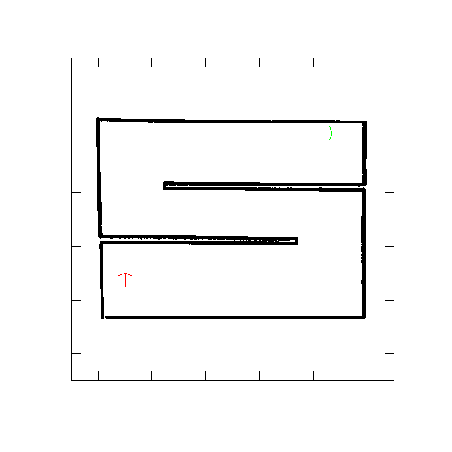
\includegraphics[scale=0.5]{./figures/slides/ch3/corridor}}%
    \gplfronttext
  \end{picture}%
\endgroup

  \vspace{0.3cm}
  \caption{\small Ο χάρτης $\bm{M}_C$ του προσομοιωμένου περιβάλλοντος CORRIDOR.
           Το πράσινο βέλος (άνω δεξιά) δείχνει την αρχική στάση του ρομπότ
           $\bm{p}_0^C$. Tο κόκκινο βέλος (κάτω αριστερά) δείχνει τη στάση-στόχο
           $\bm{p}_G^C$}
  \label{fig:02_01_03:map_corridor}
\end{figure}

\begin{figure}\centering
  % GNUPLOT: LaTeX picture with Postscript
\begingroup
  \makeatletter
  \providecommand\color[2][]{%
    \GenericError{(gnuplot) \space\space\space\@spaces}{%
      Package color not loaded in conjunction with
      terminal option `colourtext'%
    }{See the gnuplot documentation for explanation.%
    }{Either use 'blacktext' in gnuplot or load the package
      color.sty in LaTeX.}%
    \renewcommand\color[2][]{}%
  }%
  \providecommand\includegraphics[2][]{%
    \GenericError{(gnuplot) \space\space\space\@spaces}{%
      Package graphicx or graphics not loaded%
    }{See the gnuplot documentation for explanation.%
    }{The gnuplot epslatex terminal needs graphicx.sty or graphics.sty.}%
    \renewcommand\includegraphics[2][]{}%
  }%
  \providecommand\rotatebox[2]{#2}%
  \@ifundefined{ifGPcolor}{%
    \newif\ifGPcolor
    \GPcolorfalse
  }{}%
  \@ifundefined{ifGPblacktext}{%
    \newif\ifGPblacktext
    \GPblacktexttrue
  }{}%
  % define a \g@addto@macro without @ in the name:
  \let\gplgaddtomacro\g@addto@macro
  % define empty templates for all commands taking text:
  \gdef\gplfronttext{}%
  \gdef\gplfronttext{}%
  \makeatother
  \ifGPblacktext
    % no textcolor at all
    \def\colorrgb#1{}%
    \def\colorgray#1{}%
  \else
    % gray or color?
    \ifGPcolor
      \def\colorrgb#1{\color[rgb]{#1}}%
      \def\colorgray#1{\color[gray]{#1}}%
      \expandafter\def\csname LTw\endcsname{\color{white}}%
      \expandafter\def\csname LTb\endcsname{\color{black}}%
      \expandafter\def\csname LTa\endcsname{\color{black}}%
      \expandafter\def\csname LT0\endcsname{\color[rgb]{1,0,0}}%
      \expandafter\def\csname LT1\endcsname{\color[rgb]{0,1,0}}%
      \expandafter\def\csname LT2\endcsname{\color[rgb]{0,0,1}}%
      \expandafter\def\csname LT3\endcsname{\color[rgb]{1,0,1}}%
      \expandafter\def\csname LT4\endcsname{\color[rgb]{0,1,1}}%
      \expandafter\def\csname LT5\endcsname{\color[rgb]{1,1,0}}%
      \expandafter\def\csname LT6\endcsname{\color[rgb]{0,0,0}}%
      \expandafter\def\csname LT7\endcsname{\color[rgb]{1,0.3,0}}%
      \expandafter\def\csname LT8\endcsname{\color[rgb]{0.5,0.5,0.5}}%
    \else
      % gray
      \def\colorrgb#1{\color{black}}%
      \def\colorgray#1{\color[gray]{#1}}%
      \expandafter\def\csname LTw\endcsname{\color{white}}%
      \expandafter\def\csname LTb\endcsname{\color{black}}%
      \expandafter\def\csname LTa\endcsname{\color{black}}%
      \expandafter\def\csname LT0\endcsname{\color{black}}%
      \expandafter\def\csname LT1\endcsname{\color{black}}%
      \expandafter\def\csname LT2\endcsname{\color{black}}%
      \expandafter\def\csname LT3\endcsname{\color{black}}%
      \expandafter\def\csname LT4\endcsname{\color{black}}%
      \expandafter\def\csname LT5\endcsname{\color{black}}%
      \expandafter\def\csname LT6\endcsname{\color{black}}%
      \expandafter\def\csname LT7\endcsname{\color{black}}%
      \expandafter\def\csname LT8\endcsname{\color{black}}%
    \fi
  \fi
  \setlength{\unitlength}{0.0500bp}%
  \begin{picture}(3000.00,6000.00)%
    \gplgaddtomacro\gplfronttext{%
      \colorrgb{0.00,0.00,0.00}%
      \put(340,977){\makebox(0,0)[r]{\strut{}$45$}}%
      \colorrgb{0.00,0.00,0.00}%
      \put(340,1612){\makebox(0,0)[r]{\strut{}$50$}}%
      \colorrgb{0.00,0.00,0.00}%
      \put(340,2247){\makebox(0,0)[r]{\strut{}$55$}}%
      \colorrgb{0.00,0.00,0.00}%
      \put(340,2882){\makebox(0,0)[r]{\strut{}$60$}}%
      \colorrgb{0.00,0.00,0.00}%
      \put(340,3517){\makebox(0,0)[r]{\strut{}$65$}}%
      \colorrgb{0.00,0.00,0.00}%
      \put(340,4152){\makebox(0,0)[r]{\strut{}$70$}}%
      \colorrgb{0.00,0.00,0.00}%
      \put(340,4787){\makebox(0,0)[r]{\strut{}$75$}}%
      \colorrgb{0.00,0.00,0.00}%
      \put(340,5422){\makebox(0,0)[r]{\strut{}$80$}}%
      \colorrgb{0.00,0.00,0.00}%
      \put(536,440){\makebox(0,0){\strut{}$56$}}%
      \colorrgb{0.00,0.00,0.00}%
      \put(1044,440){\makebox(0,0){\strut{}$60$}}%
      \colorrgb{0.00,0.00,0.00}%
      \put(1679,440){\makebox(0,0){\strut{}$65$}}%
      \colorrgb{0.00,0.00,0.00}%
      \put(2314,440){\makebox(0,0){\strut{}$70$}}%
      \colorrgb{0.00,0.00,0.00}%
      \put(-166,3104){\rotatebox{90}{\makebox(0,0){\strut{}$y$ [m]}}}%
      \colorrgb{0.00,0.00,0.00}%
      \put(1551,110){\makebox(0,0){\strut{}$x$ [m]}}%
    }%
    \gplgaddtomacro\gplfronttext{%
    }%
    \put(0,0){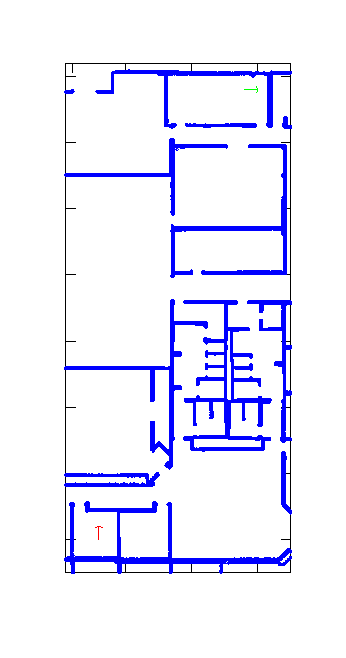
\includegraphics{./figures/parts/02/chapters/01/sections/03/willowgarage}}%
    \gplfronttext
  \end{picture}%
\endgroup

  \vspace{0.1cm}
  \caption{\small Ο χάρτης $\bm{M}_W$ τμήματος του προσομοιωμένου περιβάλλοντος
           WILLOWGARAGE. Το πράσινο βέλος (άνω δεξιά) δείχνει την αρχική στάση
           του ρομπότ $\bm{p}_0^W$. Tο κόκκινο βέλος (κάτω αριστερά) δείχνει τη
           στάση-στόχο $\bm{p}_G^W$}
  \label{fig:02_01_03:map_willowgarage}
\end{figure}

\begin{figure}\centering
  % GNUPLOT: LaTeX picture with Postscript
\begingroup
  \makeatletter
  \providecommand\color[2][]{%
    \GenericError{(gnuplot) \space\space\space\@spaces}{%
      Package color not loaded in conjunction with
      terminal option `colourtext'%
    }{See the gnuplot documentation for explanation.%
    }{Either use 'blacktext' in gnuplot or load the package
      color.sty in LaTeX.}%
    \renewcommand\color[2][]{}%
  }%
  \providecommand\includegraphics[2][]{%
    \GenericError{(gnuplot) \space\space\space\@spaces}{%
      Package graphicx or graphics not loaded%
    }{See the gnuplot documentation for explanation.%
    }{The gnuplot epslatex terminal needs graphicx.sty or graphics.sty.}%
    \renewcommand\includegraphics[2][]{}%
  }%
  \providecommand\rotatebox[2]{#2}%
  \@ifundefined{ifGPcolor}{%
    \newif\ifGPcolor
    \GPcolorfalse
  }{}%
  \@ifundefined{ifGPblacktext}{%
    \newif\ifGPblacktext
    \GPblacktexttrue
  }{}%
  % define a \g@addto@macro without @ in the name:
  \let\gplgaddtomacro\g@addto@macro
  % define empty templates for all commands taking text:
  \gdef\gplfronttext{}%
  \gdef\gplfronttext{}%
  \makeatother
  \ifGPblacktext
    % no textcolor at all
    \def\colorrgb#1{}%
    \def\colorgray#1{}%
  \else
    % gray or color?
    \ifGPcolor
      \def\colorrgb#1{\color[rgb]{#1}}%
      \def\colorgray#1{\color[gray]{#1}}%
      \expandafter\def\csname LTw\endcsname{\color{white}}%
      \expandafter\def\csname LTb\endcsname{\color{black}}%
      \expandafter\def\csname LTa\endcsname{\color{black}}%
      \expandafter\def\csname LT0\endcsname{\color[rgb]{1,0,0}}%
      \expandafter\def\csname LT1\endcsname{\color[rgb]{0,1,0}}%
      \expandafter\def\csname LT2\endcsname{\color[rgb]{0,0,1}}%
      \expandafter\def\csname LT3\endcsname{\color[rgb]{1,0,1}}%
      \expandafter\def\csname LT4\endcsname{\color[rgb]{0,1,1}}%
      \expandafter\def\csname LT5\endcsname{\color[rgb]{1,1,0}}%
      \expandafter\def\csname LT6\endcsname{\color[rgb]{0,0,0}}%
      \expandafter\def\csname LT7\endcsname{\color[rgb]{1,0.3,0}}%
      \expandafter\def\csname LT8\endcsname{\color[rgb]{0.5,0.5,0.5}}%
    \else
      % gray
      \def\colorrgb#1{\color{black}}%
      \def\colorgray#1{\color[gray]{#1}}%
      \expandafter\def\csname LTw\endcsname{\color{white}}%
      \expandafter\def\csname LTb\endcsname{\color{black}}%
      \expandafter\def\csname LTa\endcsname{\color{black}}%
      \expandafter\def\csname LT0\endcsname{\color{black}}%
      \expandafter\def\csname LT1\endcsname{\color{black}}%
      \expandafter\def\csname LT2\endcsname{\color{black}}%
      \expandafter\def\csname LT3\endcsname{\color{black}}%
      \expandafter\def\csname LT4\endcsname{\color{black}}%
      \expandafter\def\csname LT5\endcsname{\color{black}}%
      \expandafter\def\csname LT6\endcsname{\color{black}}%
      \expandafter\def\csname LT7\endcsname{\color{black}}%
      \expandafter\def\csname LT8\endcsname{\color{black}}%
    \fi
  \fi
  \setlength{\unitlength}{0.0400bp}%
  \begin{picture}(4000.00,4000.00)%
    \gplgaddtomacro\gplfronttext{%
      \colorrgb{0.00,0.00,0.00}%
      \put(388,793){\makebox(0,0)[r]{\strut{}\footnotesize $0$}}%
      \colorrgb{0.00,0.00,0.00}%
      \put(388,1158){\makebox(0,0)[r]{\strut{}\footnotesize $2$}}%
      \colorrgb{0.00,0.00,0.00}%
      \put(388,1522){\makebox(0,0)[r]{\strut{}\footnotesize $4$}}%
      \colorrgb{0.00,0.00,0.00}%
      \put(388,1887){\makebox(0,0)[r]{\strut{}\footnotesize $6$}}%
      \colorrgb{0.00,0.00,0.00}%
      \put(388,2251){\makebox(0,0)[r]{\strut{}\footnotesize $8$}}%
      \colorrgb{0.00,0.00,0.00}%
      \put(388,2616){\makebox(0,0)[r]{\strut{}\footnotesize $10$}}%
      \colorrgb{0.00,0.00,0.00}%
      \put(388,2980){\makebox(0,0)[r]{\strut{}\footnotesize $12$}}%
      \colorrgb{0.00,0.00,0.00}%
      \put(388,3345){\makebox(0,0)[r]{\strut{}\footnotesize $14$}}%
      \colorrgb{0.00,0.00,0.00}%
      \put(520,573){\makebox(0,0){\strut{}\footnotesize $6$}}%
      \colorrgb{0.00,0.00,0.00}%
      \put(885,573){\makebox(0,0){\strut{}\footnotesize $8$}}%
      \colorrgb{0.00,0.00,0.00}%
      \put(1249,573){\makebox(0,0){\strut{}\footnotesize $10$}}%
      \colorrgb{0.00,0.00,0.00}%
      \put(1614,573){\makebox(0,0){\strut{}\footnotesize $12$}}%
      \colorrgb{0.00,0.00,0.00}%
      \put(1978,573){\makebox(0,0){\strut{}\footnotesize $14$}}%
      \colorrgb{0.00,0.00,0.00}%
      \put(2343,573){\makebox(0,0){\strut{}\footnotesize $16$}}%
      \colorrgb{0.00,0.00,0.00}%
      \put(2708,573){\makebox(0,0){\strut{}\footnotesize $18$}}%
      \colorrgb{0.00,0.00,0.00}%
      \put(3072,573){\makebox(0,0){\strut{}\footnotesize $20$}}%
      \colorrgb{0.00,0.00,0.00}%
      \put(3437,573){\makebox(0,0){\strut{}\footnotesize $22$}}%
      \colorrgb{0.00,0.00,0.00}%
      \put(-118,2069){\rotatebox{90}{\makebox(0,0){\strut{}$y$ [m]}}}%
      \colorrgb{0.00,0.00,0.00}%
      \put(2069,243){\makebox(0,0){\strut{}$x$ [m]}}%
    }%
    \gplgaddtomacro\gplfronttext{%
    }%
    \put(0,0){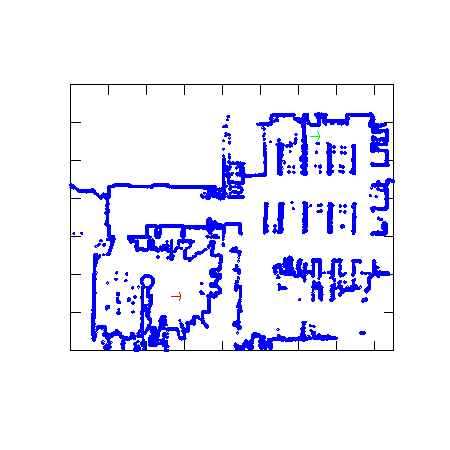
\includegraphics[scale=0.8]{./figures/slides/ch3/csal}}%
    \gplfronttext
  \end{picture}%
\endgroup

  \vspace{-0.2cm}
  \caption{\small Ο χάρτης $\bm{M}_L$ του πραγματικού περιβάλλοντος του
           εργαστηρίου Αρχιτεκτονικής Υπολογιστών του ΤΗΜΜΥ ΑΠΘ (CSAL). Το
           πράσινο βέλος (άνω δεξιά) δείχνει την αρχική στάση του ρομπότ
           $\bm{p}_0^L$. Tο κόκκινο βέλος (κάτω αριστερά) δείχνει τη στάση-στόχο
           $\bm{p}_G^L$}
  \label{fig:02_01_03:map_csal}
\end{figure}

Οι αρχικές και τελικές στάσεις ορίστηκαν έτσι ώστε να μεγιστοποιηθεί η δυσκολία
των αλγορίθμων χάραξης μονοπατιών στην εύρεση ενός εφικτού μονοπατιού και η
δυσκολία των ελεγκτών κίνησης στη διάσχισή του. Ως εκ τούτου διευκολύνουν την
έκθεση των αδυναμιών των τύπων αλγορίθμων. Οι στάσεις που τέθηκαν ως αρχικές
και τελικές συνθήκες στα τρία περιβάλλοντα καταγράφονται στον πίνακα
\ref{tbl:02_01_03:initial_and_goal_poses}.

\begin{table}[h]\centering
  \renewcommand{\arraystretch}{1.3}
  \begin{tabular}{lr}
    Στάση         & (m,m,rad)             \\ \toprule
    $\bm{p}_0^C$  & $(12.2,12.2,0.0)$     \\
    $\bm{p}_G^C$  & $(5,6.5,\pi/2)$       \\ \midrule
    $\bm{p}_0^W$  & $(69.0,79.0,0.0)$     \\
    $\bm{p}_0^W$  & $(58.0,45.0,\pi/2)$   \\ \midrule
    $\bm{p}_0^L$  & $(18.6,11.3,0.0)$     \\
    $\bm{p}_G^L$  & $(11.3,2.86,0.0)$     \\ \bottomrule
    \end{tabular}
  \caption{\small Αρχικές $\bm{p}_0$ και τελικές $\bm{p}_G$ στάσεις αυτόνομους
           πλοήγησης στα τρία περιβάλλοντα \underline{C}ORRIDOR,
           \underline{W}ILLOWGARAGE, και CSA\underline{L}}
  \label{tbl:02_01_03:initial_and_goal_poses}
\end{table}

Κάθε συνδυασμός από global και local planner δοκιμάστηκε σε κάθε περιβάλλον με
τις ίδιες αρχικές και τελικές στάσεις για $N = 10$ φορές, και επομένως η
αξιολόγηση των απόδοσης όλων των συνδυασμών έγινε με τη χρήση στατιστικών
μέσων. Κάθε συνδυασμός έλαβε μια χρονική περίοδο για να εκτελέσει την πλοήγησή
του από την αρχή ως τον στόχο, η οποία ορίστηκε σε $t_C^{max} = 120$ sec για
τον κόσμο CORRIDOR, $t_W^{max} = 180$ sec για τον κόσμο WILLOWGARAGE, και
$t_L^{max} = 600$ sec στο περιβάλλον CSAL.

Όλες οι προσομοιώσεις πραγματοποιήθηκαν στο λειτουργικό σύστημα Linux Ubuntu
16.04, σε υπολογιστή με επεξεργαστή 12 νημάτων, 32GB μνήμης, και συχνότητα
ρολογιού $4.00$ GHz. Όλα τα πειράματα που πραγματοποιήθηκαν στο περιβάλλον CSAL
πραγματοποιήθηκαν σε Linux Ubuntu 16.04, σε υπολογιστή με επεξεργαστή με 4
νήματα, $8$ GB μνήμης, και συχνότητα ρολογιού $3.20$ GHz.



%%%%%%%%%%%%%%%%%%%%%%%%%%%%%%%%%%%%%%%%%%%%%%%%%%%%%%%%%%%%%%%%%%%%%%%%%%%%%%%%
\subsection{Ορισμός μετρικών αξιολόγησης}
\label{subsection:02_01_03:02}

Σε αυτήν την ενότητα κάνουμε τις ακόλουθες παραδοχές και ορισμούς.

\begin{bw_box}
\begin{definition}
Ένα μονοπάτι $\bm{P} : [1,n] \rightarrow \mathbb{R}^2 \times [-\pi, \pi)$ είναι
μια ακολουθία στάσεων $\bm{p}_i, i = 1,2,\dots,n$, δηλαδή
$\bm{P} \equiv \{\bm{p}_1, \bm{p}_2, \dots, \bm{p}_n\}$, όπου
$\bm{p}_i = (x_i, y_i, \theta_i)$, είναι οι συντεταγμένες μίας στάσης στον
$\mathbb{R}^2$ και $\theta_i$ είναι ο προσανατολισμός του διανύσματος που
ξεκινά από το σημείο $(x_i,y_i)$ ως προς τον άξονα $x$ του συστήματος αναφοράς
του χάρτη.
\end{definition}
\end{bw_box}

Το μέγεθος (cardinality) του $\bm{P}$ αναφέρεται ως $|\bm{P}|$ και
είναι ίσο με τον αριθμό των στάσεων του $\bm{P}$. Συμβολίζουμε μία συλλογή $N$
μονοπατιών $\bm{P}_j$, $j = 1,2,\dots,N$ με $\bm{\mathcal{P}} = \{\bm{P}_1,
\bm{P}_2, \dots, \bm{P}_N\}$.

\begin{bw_box}
\begin{definition}
Η απόσταση μεταξύ δύο στάσεων $\bm{p}_i$ και $\bm{p}_j$ είναι η
Ευκλείδεια απόσταση $d\bm{(p}_i,\bm{p}_j) = ((x_i - x_j)^2 + (y_i - y_j)^2)^{1/2}$.
\end{definition}
\end{bw_box}

\begin{bw_box}
\begin{definition}
Ένας χάρτης πλέγματος πληρότητας (Occupancy Grid Map---OGM)
$\bm{M} : [1, q] \rightarrow \mathbb{R}^2$ είναι ένα
μη ταξινομημένο σύνολο σημείων στο καρτεσιανό επίπεδο:
$\bm{M} \equiv ((x_1^M, y_1^M), (x_2^M, y_2^M), \dots, (x_q^M, y_q^M) )$.
\end{definition}
\end{bw_box}

\begin{bw_box}
\begin{definition}
Το μήκος ενός μονοπατιού $\bm{P}$ συμβολίζεται με $l(\bm{P})$ και υπολογίζεται
ως:
\begin{align}
  l(\bm{P}) = \sum\limits_{i=1}^{|\bm{P}|-1} d(p_i, p_{i+1})
  \label{eq:path_length}
\end{align}
δηλαδή είναι το άθροισμα των αποστάσεων μεταξύ διαδοχικών θέσεων
  $\bm{p}_i$ και $\bm{p}_{i+1}$.
\end{definition}
\end{bw_box}

\begin{bw_box}
\begin{definition}
Η ομαλότητα ενός μονοπατιού $\bm{P}$, $s(\bm{P})$, ορίζεται ως:
\begin{align}
  s(\bm{P}) = \Big(\dfrac{1}{|\bm{P}|-2}\sum\limits_{i=1}^{|\bm{P}|-1} (\theta_{i+1} - \theta_i)^2\Big)^{1/2}
  \label{eq:path_smoothness}
\end{align}
\end{definition}
\end{bw_box}

\begin{bw_box}
\begin{definition}
Η μέση ελάχιστη απόσταση ενός μονοπατιού $\bm{P}$ από τα εμπόδια του χάρτη
$\bm{M}$ είναι η μέση απόσταση των στάσεων που αποτελούν το μονοπάτι από το
πλησιέστερο εμπόδιο της κάθε μίας. Συμβολίζεται με $d(\bm{P},\bm{M})$ και
ορίζεται ως:
\begin{align}
  d(\bm{P},\bm{M}) = \dfrac{1}{|\bm{P}|} \sum\limits_{k=1}^{|\bm{P}|} \min\limits_{i=1,2,\dots,q} d(\bm{p}_k,\bm{m}_i)
  \label{eq:mean_min_obs_dist}
\end{align}

όπου $\bm{p}_k \in \bm{P}$, $k = 1,2,\dots,|\bm{P}|$, και
$\bm{m}_i \in \bm{M}$, $i = 1,2,\dots,q$.
\end{definition}
\end{bw_box}

\begin{bw_box}
\begin{definition}
Η ολική ελάχιστη απόσταση μιας συλλογής μονοπατιών
$\bm{\mathcal{P}} = \{ \bm{P}_1, \bm{P}_2, \dots, \bm{P}_N \}$ από τα εμπόδια
του $\bm{M}$ συμβολίζεται με $\inf(d(\bm{\mathcal{P}},\bm{M}))$ (για να
επισημανθεί η απόλυτη φύση αυτής της ελάχιστης τιμής), και ορίζεται ως:
\begin{align}
  \inf(d(\mathcal{P},\bm{M})) = \min\limits_{j=1,2,\dots,N} \big\{ \min\limits_{\substack{k=1,2,\dots, |\bm{P}_j| \\ i=1,2,\dots,q}} d(\bm{p}_k^j,\bm{m}_i) \big\}
  \label{eq:abs_min_obs_dist}
\end{align}

όπου $\bm{P}_j \in \mathcal{P}$, $\bm{p}_k^j \in \bm{P}_j$,
$k = 1,2,\dots,|\bm{P}_j|$, και $\bm{m}_i \in \bm{M}$, $i =1,2,\dots,q$.
\end{definition}
\end{bw_box}

\begin{bw_box}
\begin{definition}
Η μέση απόκλιση ενός μονοπατιού $\bm{P}_1$ από ένα μονοπάτι $\bm{P}_2$
υπολογίζεται ως η μέση απόσταση κάθε στάσης του $\bm{P}_1$ από την πλησιέστερη
στάση της που ανήκει στο $\bm{P}_2$:
\begin{align}
  d_{\delta}(\bm{P}_1,\bm{P}_2) = \dfrac{1}{|\bm{P}_1|} \sum\limits_{k=1}^{|\bm{P}_1|} \min\limits_{l=1,2,\dots,|\bm{P}_2|} d(\bm{p}_k, \bm{p}_l)
\end{align}

όπου $\bm{p}_k \in \bm{P}_1$, $k = 1,2,\dots,|\bm{P}_1|$, και
$\bm{p}_l \in \bm{P}_2$, $l = 1,2,\dots,|\bm{P}_2|$.
\end{definition}
\end{bw_box}

\begin{bw_box}
\begin{definition}
Η ολική απόκλιση ενός μονοπατιού $\bm{P}_1$ από ένα μονοπάτι $\bm{P}_2$
υπολογίζεται ως το άθροισμα της απόστασης κάθε στάσης που αποτελεί το $\bm{P}_1$
από την πλησιέστερη στάση της στο $\bm{P}_2$:
\begin{align}
  d_{\Delta}(\bm{P}_1,\bm{P}_2) = |\bm{P}_1| \cdot d_{\delta}(\bm{P}_1,\bm{P}_2)
\end{align}
\end{definition}
\end{bw_box}


Η μετρική απόστασης Frechet, η οποία εισήχθη από τον Maurice Frechet για
συνεχείς καμπύλες σε ένα μετρικό χώρο το 1906 \cite{Frechet1906}, είναι ένα
μέτρο της ομοιότητας μεταξύ δύο καμπυλών. Στα πλαίσια της διατριβής προτιμάται
από την μετρική απόστασης Pompeiu-Hausdorff \cite{RockafellarR} λόγω του ότι η
τελευταία δεν λαμβάνει υπόψη της τη θέση και τη διάταξη των σημείων κατά μήκος
μιας καμπύλης (εν προκειμένω ενός μονοπατιού).


\begin{bw_box}
\begin{definition}
Για διακριτές καμπύλες
$\bm{P}_1 : [1, m] \rightarrow V$ και $\bm{P}_2 : [1, n] \rightarrow V$
(όπως τα δείγματα στάσης ενός μονοπατιού και τα ολικά μονοπάτια) που
αποτελούνται από ακολουθίες διακριτών σημείων
$\lambda(\bm{P}_1) \equiv \{\bm{P}_1(1),\ \ \bm{P}_1(2),\ \ \dots\ \bm{P}_1(m)\} \equiv \{v_1, v_2, \dots v_p\}$ και
$\lambda(\bm{P}_2) \equiv \{\bm{P}_2(1),\ \ \bm{P}_2(2),\ \ \dots\ \bm{P}_2(n)\} \equiv \{u_1, u_2, \dots u_g\}$
αντίστοιχα, η διακριτή απόσταση Frechet ορίζεται ως:
\begin{align}
  \delta_{d}^F(\bm{P}_1,\bm{P}_2) = \min\{ &\|\bm{L}\| \ | \ \bm{L} \text{ είναι μια σύζευξη μεταξύ } \bm{P}_1 \text{ και } \bm{P}_2 \}
\end{align}

όπου $\|\bm{L}\| = \max\limits_{i=1,\dots q} d(\bm{u}_{a_i}, \bm{u}_{b_i})$.
Μια σύζευξη $\bm{L}$ είναι μια ακολουθία διαφορετικών ζευγών από το
$\lambda(\bm{P}_1) \times \lambda(\bm{P}_2)$: $L \equiv \}(\bm{u}_{a_1},
\bm{v}_{b_1}), (\bm{u}_{a_2}, \bm{v}_{b_2}), \dots , (\bm{u}_{a_q},
\bm{v}_{b_q})\}$, και $d(\bm{a},\bm{b})$ είναι ένα μετρική της απόστασης (εδώ
ίση με την ευκλείδεια απόσταση όπως ορίζεται παραπάνω) μεταξύ των σημείων
$\bm{a}$ και $\bm{b}$.

\end{definition}
\end{bw_box}

Επιπλέον, έστω ότι συμβολισμοί $\mu(x),\sigma(x)$ να υποδηλώνουν τη μέση τιμή
και την τυπική απόκλιση της μεταβλητής $x$.  Συμβολίζοντας με
$\bm{\mathcal{G}}$ μια συλλογή από $N$ συνολικά μονοπάτια προς ακολούθηση που
παράγονται σε $N$ πειράματα και προσομοιώσεις που πραγματοποιήθηκαν,
$\bm{\mathcal{G}} = \{ \bm{G}_1, \bm{G}_2, \dots, \bm{G}_N \}$, και με
$\bm{\mathcal{P}}$ μια συλλογή από $N$ διανυόμενες διαδρομές $\bm{\mathcal{P}}
= \{ \bm{P}_1, \bm{P}_2, \dots, \bm{P}_N \}$, οι μετρικές αξιολόγησης για τους
κατασκευαστές μονοπατιών global planners, τους ελεγκτές κίνησης local planners,
και τους συνδυασμούς τους παρουσιάζονται στους πίνακες
\ref{tbl:metrics_and_proportionality_global_planners},
\ref{tbl:metrics_and_proportionality_local_planners}, και
\ref{tbl:metrics_and_proportionality_combination_planners}.


\begin{table}[h]\hspace{-2.5cm}
  \renewcommand{\arraystretch}{1.8}
  \begin{tabular}{rcc}
    \begin{minipage} [t]{0.25\columnwidth}Μετρική αξιολόγησης \\ global planner \\ \end{minipage} & Τύπος & \begin{minipage} [t]{0.2\columnwidth}Τύπος \\ αναλογικότητας \\ \end{minipage} \\ \toprule
    $\mu_{l}(\bm{\mathcal{G}})$ &
    \begin{minipage}[t]{0.7\columnwidth}%
      Το μέσο μήκος των συνολικών σχεδιασθέντων μονοπατιών
      $\mu_l(\bm{\mathcal{G}}) = \mu(l(\bm{G}_j))$ [m], $j = 1,2,\dots,N$
    \end{minipage} & $\searrow$ \\
    $\sigma_{l}(\bm{\mathcal{G}})$ &
    \begin{minipage}[t]{0.7\columnwidth}%
      Η τυπική απόκλιση γύρω από το μέσο μήκος μονοπατιών
      $\sigma_l(\bm{\mathcal{G}}) = \sigma(l(\bm{G}_j))$ [m],
      $j = 1,2,\dots,N$---ένα μέτρο της συνέπειας σχεδιασμού μονοπατιών
    \end{minipage} & $\searrow$ \\
    $\mu_r(\bm{\mathcal{G}})$ &
    \begin{minipage}[t]{0.7\columnwidth}%
      Ο μέσος αριθμός των στάσεων του συνολικού μονοπατιού επί του μέσου μήκους
      του συνολικού μονοπατιού
      $\mu_r(\bm{\mathcal{G}}) = \mu(|\bm{G}_j| / l(\bm{\bm{G}_j}))$
      [θέσεις / m], $j = 1,2,\dots,N$---ένα μέτρο της αναλυτικότητας μονοπατιών:
      όσο υψηλότερη η ανάλυση, τόσο λεπτομερέστερα τα μονοπάτια και τόσο
      λεπτότεροι οι ελιγμοί του ρομπότ (εάν, για παράδειγμα, το απαιτούν οι
      προδιαγραφές)
    \end{minipage} & $\nearrow$ \\
    $\mu_{s}(\bm{\mathcal{G}})$ &
    \begin{minipage}[t]{0.7\columnwidth}%
      Η μέση ομαλότητα των παραγόμενων μονοπατιών
      $\mu_s(\bm{\mathcal{G}}) = \mu(s(\bm{G}_j))$ [rad], $j = 1,2,\dots,N$
    \end{minipage} &
    $\searrow$ \\
    $\sigma_{s}(\bm{\mathcal{G}})$ &
    \begin{minipage}[t]{0.7\columnwidth}%
      Η τυπική απόκλιση γύρω από τη μέση ομαλότητα σχεδιασθέντων μονοπατιών
      $\sigma_s(\bm{\mathcal{G}}) = \sigma(s(\bm{G}_j))$ [rad], $j = 1,2,\dots,N$
    \end{minipage} & $\searrow$ \\
    $\inf(d(\bm{\mathcal{G}},\bm{M}))$ &
    \begin{minipage}[t]{0.7\columnwidth}%
      Η συνολική ελάχιστη απόσταση σχεδιασθέντων μονοπατιών από τα εμπόδια του
      χάρτη $\bm{M}$
      $\inf(d(\bm{\mathcal{G}},\bm{M}))$ [m]---ένα μέτρο του πόσο καλή είναι
      η σχεδίαση ενός μονοπατιού με βάση την απόσταση από εμπόδια του χάρτη
    \end{minipage} & $\nearrow$ \\
    $\mu(d(\bm{\mathcal{G}}, \bm{M}))$ &
    \begin{minipage}[t]{0.7\columnwidth}%
      Η μέση ελάχιστη απόσταση των σχεδιασθέντων μονοπατιών από τα εμπόδια του
      χάρτη $\bm{M}$, $\mu(d(\bm{G}_j,\bm{M}))$ [m], $j = 1,2,\dots,N$
    \end{minipage} & $\nearrow$ \\
    $\sigma(d(\bm{\mathcal{G}},\bm{M}))$ &
    \begin{minipage}[t]{0.7\columnwidth}%
      Η τυπική απόκλιση γύρω από τη μέση ελάχιστη απόσταση των μονοπατιών
      από τα εμπόδια του χάρτη $\bm{M}$, $\sigma(d(\bm{G}_j,\bm{M}))$ [m],
      $j = 1,2,\dots,N$
    \end{minipage} & $\searrow$ \\ \bottomrule
  \end{tabular}
  \caption{\small Μετρικές αξιολόγησης για τους αλγορίθμους κατασκευής μονοπατιών
           (global planners) (αριστερά), η περιγραφή τους (μέση) και η φύση
           της συμβολής τους στην τιμήαξία ενός συνδυασμού αλγορίθμων για
           αυτόνομη πλοήγηση (δεξιά): τα βέλη που δείχνουν προς τα πάνω
           υποδηλώνουν ότι όσο υψηλότερη είναι η τιμή μιας μετρικής τόσο
           υψηλότερη είναι η αξία του συνδυασμού. Tα βέλη που δείχνουν προς τα
           κάτω υποδεικνύουν ότι η αξία ενός συνδυασμού είναι τόσο υψηλότερη
           όσο χαμηλότερη είναι η τιμή της εν λόγω μετρικής}
  \label{tbl:metrics_and_proportionality_global_planners}
\end{table}

\begin{table}\hspace{-2.5cm}
  \renewcommand{\arraystretch}{1.8}
  \begin{tabular}{rcc}
    \begin{minipage} [t]{0.25\columnwidth}Μετρική αξιολόγησης \\ local planner \\ \end{minipage} & Τύπος & \begin{minipage} [t]{0.2\columnwidth}Τύπος \\ αναλογικότητας \\ \end{minipage} \\ \toprule
    $\mu_{A} / N$ &
    \begin{minipage}[t]{0.7\columnwidth}%
      Ο μέσος αριθμός των ματαιωμένων αποστολών επί του συνολικού αριθμού των
      προσομοιώσεων ή πειραμάτων που πραγματοποιήθηκαν
    \end{minipage} & $\searrow$ \\
    $\mu_{RR}$ &
    \begin{minipage}[t]{0.7\columnwidth}%
      Ο μέσος αριθμός των ανακτήσεων με περιστροφή
    \end{minipage} & $\searrow$ \\
    $\sigma_{RR}$ &
    \begin{minipage}[t]{0.7\columnwidth}%
      Η τυπική απόκλιση γύρω από τον μέσο αριθμό των ανακτήσεων με περιστροφή
    \end{minipage} & $\searrow$ \\
    $\mu_{CC}$ &
    \begin{minipage}[t]{0.7\columnwidth}%
      Ο μέσος αριθμός των εκκαθαρίσεων του χάρτη κόστους
    \end{minipage} & $\searrow$ \\
    $\sigma_{CC}$ &
    \begin{minipage}[t]{0.7\columnwidth}%
      Η τυπική απόκλιση γύρω από τον μέσο αριθμό των εκκαθαρίσεων του χάρτη
      κόστους
    \end{minipage} & $\searrow$ \\
    $\mu_{PF}$ &
    \begin{minipage}[t]{0.7\columnwidth}%
      Ο μέσος αριθμός αποτυχιών διαδρομής---ένα μέτρο του πόσες φορές ο ελεγκτής
      κίνησης απέτυχε να υπολογίσει έγκυρες ταχύτητες κίνησης
    \end{minipage} & $\searrow$ \\
    $\sigma_{PF}$ &
    \begin{minipage}[t]{0.7\columnwidth}%
      Η τυπική απόκλιση γύρω από το μέσο αριθμό αποτυχιών διαδρομής
    \end{minipage} & $\searrow$ \\
    $\mu_{PF} / \mu_{LPC}$ &
    \begin{minipage}[t]{0.7\columnwidth}%
      Ο μέσος αριθμός αποτυχιών διαδρομής επί του μέσου αριθμού κλήσεων του
      ελεγκτή κίνησης--- ένα μέτρο του πόσο συχνά ο τοπικός σχεδιαστής απέτυχε
      να ελέγξει την τροχιά του ρομπότ
    \end{minipage} & $\searrow$ \\ \bottomrule
  \end{tabular}
  \caption{\small Μετρικές αξιολόγησης για τους ελεγκτές κίνησης
           (local planners) (αριστερά), η περιγραφή τους (μέση) και η φύση
           της συμβολής τους στην τιμή-αξία ενός συνδυασμού αλγορίθμων για
           αυτόνομη πλοήγηση (δεξιά): τα βέλη που δείχνουν προς τα πάνω
           υποδηλώνουν ότι όσο υψηλότερη είναι η τιμή μιας μετρικής τόσο
           υψηλότερη είναι η αξία του συνδυασμού. Tα βέλη που δείχνουν προς τα
           κάτω υποδεικνύουν ότι η αξία ενός συνδυασμού είναι τόσο υψηλότερη
           όσο χαμηλότερη είναι η τιμή της εν λόγω μετρικής}
  \label{tbl:metrics_and_proportionality_local_planners}
\end{table}

\begin{table}\hspace{-2.5cm}
  \renewcommand{\arraystretch}{1.8}
  \begin{tabular}{rcc}
    \begin{minipage} [t]{0.25\columnwidth} Μετρική αξιολόγησης \\ συνδυασμών global \\ και local planner \\ \end{minipage}  & Τύπος & \begin{minipage} [t]{0.2\columnwidth}Τύπος \\ αναλογικότητας \\ \end{minipage} \\ \toprule
    $\mu_{\delta}(\bm{\mathcal{P}},\bm{\mathcal{G}})$ &
    \begin{minipage}[t]{0.7\columnwidth}%
      Η μέση απόκλιση μεταξύ των πραγματικών διαδρομών $\bm{\mathcal{P}}$ που
      ακολούθησε το ρομπότ σε σύγκριση με τα σχεδιασθέντα μονοπάτια
      $\bm{\mathcal{G}}$ που επρόκειτο να ακολουθήσει
      $\mu_{\delta}(\bm{\mathcal{P}},\bm{\mathcal{G}}) = \mu(d_{\delta}(\bm{P}_j, \bm{G}_j))$ [m],
      $j = 1,2,\dots,N$
      \end{minipage} & $\searrow$ \\
    $\mu_{\Delta}(\bm{\mathcal{P}},\bm{\mathcal{G}})$ &
    \begin{minipage}[t]{0.7\columnwidth}%
      Η μέση συνολική απόκλιση μεταξύ των πραγματικών διαδρομών
      $\bm{\mathcal{P}}$ που ακολούθησε το ρομπότ σε σύγκριση με τα σχεδιασθέντα
      μονοπάτια $\bm{\mathcal{G}}$ που επρόκειτο να ακολουθήσει
      $\mu_{\Delta}(\bm{\mathcal{P}},\bm{\mathcal{G}}) = \mu(d_{\Delta}(\bm{P}_j, \bm{G}_j))$ [m],
      $j = 1,2,\dots,N$
      \end{minipage} & $\searrow$ \\
    $\mu_{\delta}^F(\bm{\mathcal{P}},\bm{\mathcal{G}})$ &
    \begin{minipage}[t]{0.7\columnwidth}%
      Η μέση απόσταση Frechet μεταξύ των πραγματικών διαδρομών
      $\bm{\mathcal{P}}$ που ακολούθησε το ρομπότ και των αντίστοιχων
      σχεδιασθέντων μονοπατιών $\bm{\mathcal{G}}$,
      $\mu_{\delta}^F(\bm{\mathcal{P}},\bm{\mathcal{G}}) = \mu(\delta_{dF}(\bm{P}_j, \bm{G}_j))$ [m],
      $j = 1,2,\dots,N$
      \end{minipage} & $\searrow$ \\
    $\mu_{t}$ &
    \begin{minipage}[t]{0.7\columnwidth}%
      Ο μέσος χρόνος διαδρομής από την αρχική στάση $\bm{p}_0$ στη στάση-στόχο
      $\bm{p}_G$ [sec]
      \end{minipage} & $\searrow$ \\
    $\sigma_{t}$ &
    \begin{minipage}[t]{0.7\columnwidth}%
      Η τυπική απόκλιση γύρω από το μέσο χρόνο διαδρομής [sec]
      \end{minipage} & $\searrow$ \\
    $\mu_{l}(\bm{\mathcal{P}})$ &
    \begin{minipage}[t]{0.7\columnwidth}%
      Το μέσο μήκος των πραγματικών διαδρομών $\bm{\mathcal{P}}$ που ακολούθησε
      το ρομπότ ως αποτέλεσμα του ελεγκτή κίνησης
      $\mu_l(\bm{\mathcal{P}}) = \mu(l(\bm{P}_j))$ [m], $j = 1,2,\dots,N$
      \end{minipage} & $\searrow$ \\
    $\sigma_{l}(\bm{\mathcal{P}})$ &
    \begin{minipage}[t]{0.7\columnwidth}%
      Η τυπική απόκλιση γύρω από το μέσο πραγματικό μήκος διαδρομής
      $\sigma_l(\bm{\mathcal{P}}) = \sigma(l(\bm{P}_j))$ [m],
      $j = 1,2,\dots,N$---ένα μέτρο της συνέπειας των διαδρομών που υπαγόρευσε
      ο ελεγκτής κίνησης στο ρομπότ
      \end{minipage} & $\searrow$ \\
    $\mu_{s}(\bm{\mathcal{P}})$ &
    \begin{minipage}[t]{0.7\columnwidth}%
      Η μέση ομαλότητα των διανυόμενων διαδρομών
      $\mu_s(\bm{\mathcal{P}}) = \mu(s(\bm{P}_j))$ [rad], $j = 1,2,\dots,N$
      \end{minipage} & $\searrow$ \\
    $\sigma_{s}(\bm{\mathcal{P}})$ &
    \begin{minipage}[t]{0.7\columnwidth}%
      Η τυπική απόκλιση γύρω από τη μέση ομαλότητα των διανυόμενων διαδρομών
      $\sigma_s(\bm{\mathcal{P}}) = \sigma(s(\bm{P}_j))$ [rad], $j = 1,2,\dots,N$
      \end{minipage} & $\searrow$ \\
    $\inf(d(\bm{\mathcal{P}},\bm{M}_C))$ &
    \begin{minipage}[t]{0.7\columnwidth}%
      Η συνολική ελάχιστη απόσταση των πραγματικών διαδρομών που ακολούθησε το
      ρομπότ από τα εμπόδια του χάρτη $\bm{M}$ σε όλα τα πειράματα ή τις
      προσομοιώσεις $\inf(d(\bm{\mathcal{P}}, \bm{M}))$ [m]---ένα μέτρο του πόσο
      καλά ο ελεγκτής κίνησης σχεδιάζει και εκτελεί τη διαδρομή του ρομπότ γύρω
      από τα εμπόδια ώστε να μην παραβιάζει περιορισμούς αποφυγής σύγκρουσης
      \end{minipage} & $\nearrow$ \\
    $\mu(d(\bm{\mathcal{P}},\bm{M}_C))$ &
    \begin{minipage}[t]{0.7\columnwidth}%
      Η μέση ελάχιστη απόσταση των πραγματικών διαδρομών που διέσχισε το
      ρομπότ από τα εμπόδια του χάρτη $\bm{M}$, $\mu(d(\bm{P}_j, \bm{M}))$ [m],
      $j = 1,2,\dots,N$
      \end{minipage} & $\nearrow$ \\
    $\sigma(d(\bm{\mathcal{P}},\bm{M}_C))$ &
    \begin{minipage}[t]{0.7\columnwidth}%
      Η τυπική απόκλιση γύρω από τη μέση ελάχιστη απόσταση των πραγματικών
      διαδρομών του ρομπότ από τα εμπόδια του χάρτη $\bm{M}$,
      $\sigma(d(\bm{P}_j, \bm{M}))$ [m], $j = 1,2,\dots,N$
      \end{minipage} & $\searrow$ \\ \bottomrule
  \end{tabular}
  \caption{\small Μετρικές αξιολόγησης για τον συνδυασμό ενός αλγορίθμου
           χάραξης μονοπατιών (global planner) με έναν ελεγκτή κίνησης
           (local planner), η περιγραφή τους (μέση) και η φύση της συμβολής
           τους στην τιμή-αξία του συνδυασμού τους (δεξιά): τα βέλη που δείχνουν
           προς τα πάνω υποδηλώνουν ότι όσο υψηλότερη είναι η τιμή μιας
           μετρικής τόσο υψηλότερη είναι η αξία του συνδυασμού. Τα βέλη που
           δείχνουν προς τα κάτω υποδεικνύουν ότι η αξία ενός συνδυασμού τόσο
           υψηλότερη όσο χαμηλότερη είναι η τιμή της εν λόγω μετρικής}
  \label{tbl:metrics_and_proportionality_combination_planners}
\end{table}



%%%%%%%%%%%%%%%%%%%%%%%%%%%%%%%%%%%%%%%%%%%%%%%%%%%%%%%%%%%%%%%%%%%%%%%%%%%%%%%%
\subsection{Μεθοδολογία συνολικής και ιεραρχημένης αξιολόγησης}
\label{subsection:02_01_03:03}

Η συνολική αξιολόγηση κάθε συνδυασμού global και local planner πραγματοποιείται
με βάση την κοινή τους επίδοση και τις επιδόσεις των δύο συνιστωσών του. Κάθε
μετρική $m$ που περιγράφεται ανωτέρω λαμβάνεται υπόψη και της αποδίδεται ένα
βάρος $w_m \in \mathbb{R}_{\ge 0}$, έτσι ώστε η γενική αξιολόγηση να είναι
εφικτή για μεταβλητές προδιαγραφές (ανάλογα με την εφαρμογή, ένας μηχανικός
μπορεί να προτιμήσει να αποδώσει περαιτέρω σημασία, για παράδειγμα, στο μήκος
των διαδρομών του σε σχέση με το συνολικό χρόνο πλοήγησης). Απώτερος στόχος
είναι η απόδοση μίας τιμής-αξίας σε κάθε συνδυασμό αλγορίθμων πλοήγησης, η
οποία θα τους διακρίνει και θα τους κατατάσσει με βάση της συνολική τους
επίδοση.

Αρχικά κάνουμε την παραδοχή ότι η τιμή ενός συνδυασμού πρέπει να είναι αυστηρά
αύξουσα, έτσι ώστε οι μεγαλύτερες τιμές να αντικατοπτρίζουν καλύτερες
επιδόσεις. Η τιμή αυτή εξαρτάται όχι μόνο από την τιμή κάθε μετρικής που
συζητήθηκε μέχρι τώρα, αλλά, πιο συγκεκριμένα, από τη φύση της συμβολής μιας
μετρικής. Για παράδειγμα, οι χρόνοι πλοήγησης μεταξύ $p_0^{\bm{M}_C}$ και
$p_G^{\bm{M}_C}$ συμβάλλουν περισσότερο όσο μικρότερη είναι η τιμή τους, αλλά,
σε σχέση με τη συνολική απόσταση μεταξύ των εμποδίων, η τιμή ενός συνδυασμού θα
πρέπει να αυξάνεται όσο μεγαλύτερη είναι αυτή η απόσταση. Επομένως, η τιμή ενός
συνδυασμού αλγορίθμων εξαρτάται από τον τύπο της αναλογικότητας της συνεισφοράς
κάθε συγκεκριμένης μετρικής. Οι πίνακες
\ref{tbl:metrics_and_proportionality_global_planners}-\ref{tbl:metrics_and_proportionality_combination_planners}
συνοψίζουν τη συμβολή κάθε μετρικής που αφορά τους αλγορίθμους κατασκευής
μονοπατιών, τους ελεγκτές κίνησης, και του συνδυασμού τους. Τα βέλη που
δείχνουν προς τα πάνω υποδηλώνουν ευθεία αναλογικότητα. Τα βέλη που δείχνουν
προς τα κάτω υποδηλώνουν αντίστροφη αναλογικότητα. Περισσότερες λεπτοµέρειες
υπάρχουν στο παράρτηµα \ref{appendix:proportionality_contribution}.

Δεδομένου ότι αυτό που επιδιώκουμε είναι η απόδοση μιας κλιμακωτής τιμής $V(C)$ σε
κάθε συνδυασμό $C$ από αλγορίθμους σχεδιασμού μονοπατιών και ελεγκτών κίνησης,
πρέπει να περάσουμε από την κατασκευή μιας έγκυρης συνάρτησης αξίας $V$. Η
συνάρτηση $V$ πρέπει (α) να είναι γνησίως αύξουσα (ώστε να εκφράζει με ακρίβεια
την αξία ενός συνδυασμού με βάση τις μετρικές επίδοσης του, και ταυτόχρονα να
παρέχει ένα νόημα στις διαφορές τους, η οποία να μπορεί να αναχθεί στη διαφορά
μεταξύ της επίδοσης ξεχωριστών μετρικών τους) και (β) να λαμβάνει υπόψη
μετρικές διαφορετικών μονάδων μέτρησης. Για τον σκοπό αυτό ξεκινάμε με την
κανονικοποίηση των τιμών των μετρικών εντός του αντίστοιχου διαστήματος
ελάχιστων και μέγιστων τιμών για όλους τους συνδυασμούς---έτσι ώστε η τιμή όλων
των μετρικών να εκφράζεται στο διάστημα $[0,1]$ άνευ μονάδας μέτρησης---και
ανάλογα με τα συμφραζόμενα. Το τελευταίο σημαίνει ότι η τιμή, για παράδειγμα,
του μέσου μήκους $N$ σχεδίων μονοπατιών θα εκφράζεται μεταξύ του ελάχιστου μέσου
μήκους και του μέγιστου μέσου μήκους όλων των μονοπατιών και όλων των
συνδυασμών---αφού αυτή η μετρική είναι ανεξάρτητη από την επιτυχία ή την
αποτυχία της αποστολής ενός συνδυασμού---, αλλά ο μέσος χρόνος πλοήγησης μεταξύ
$\bm{p}_0^M$ και $\bm{p}_G^M$ στον χάρτη $\bm{M}$, ο οποίος εξαρτάται από την
επιτυχία της αποστολής, θα εκφράζεται μόνο μεταξύ του ελάχιστου μέσου και του
μέγιστου μέσου χρόνου διαδρομής των συνδυασμών που κατάφεραν να μεταφέρουν το
ρομπότ από τη στάση $\bm{p}_0^M$ στην ${p}_G^M$. Η κανονικοποιητική συνάρτηση
για μία μετρική $m$ είναι $N(m)$:
\begin{align}
  N(m) &= \dfrac{m - \min m}{\max m - \min m}
\end{align}

Έστω $S$ το σύνολο των συνδυασμών $C$ που κατάφεραν να κάνουν το ρομπότ να
πλοηγηθεί από τη στάση $\bm{p}_0^M$ στην $\bm{p}_G^M$ για τον χάρτη $\bm{M}$.
Έστω $D$ το σύνολο των μετρικών που δεν εξαρτώνται από την επιτυχία μιας
αποστολής (με την παραπάνω έννοια), δηλαδή μετρικές που αφορούν αποκλειστικά σε
global και local planners αλλά όχι στο συνδυασμό τους. Έστω επίσης η
συνάρτηση-δείκτης (indicator function) $I_A(x)$ για τη μετρική $x$ και το
σύνολο $A$: η $I_A(x)$ ισούται με ένα αν $x \in A$ και με μηδέν αλλιώς. Τότε η
συνάρτηση δείκτης για το συνδυασμό $C$ όσον αφορά στη μετρική $m$,
$I(C,m) = I_S(C)\ ||\ I_D(m)$, είναι μηδέν όταν ο $C$ ήταν ανεπιτυχής στην
αποστολή του και $m$ είναι μετρική που αφορά το συνδυασμό αλγορίθμων---σε
όλες τις άλλες περιπτώσεις η $I(C,m)$ ισούται με ένα. Η διατύπωση αυτής της
συνάρτησης δείκτη με τέτοιο τρόπο καθιστά δυνατή τη συνεκτίμηση όλων των
μετρικών που περιγράφηκαν μέχρι σε αυτό το σημείο, και μέσω αυτής ο υπολογισμός
της $V$ είναι εφικτός.

Για τους αλγορίθμους παραγωγής μονοπατιών, τους ελεγκτές κίνησης, ή τους
συνδυασμούς τους, εάν η τιμή τους όσον αφορά στη μετρική $m$ είναι ευθέως
ανάλογη της τιμής της $m$ (όπως η τιμή της μετρικής της συνολικής ελάχιστης
απόστασης του ρομπότ από τα εμπόδια), η τιμή-αξία που αποδίδεται σε έναν
αλγόριθμο, ελεγκτή, ή συνδυασμό τους $C$ για τη μετρική $m$ εκφράζεται στο
διάστημα $\mathbb{R}_{\ge 0} \times [0,1]$ και εκφράζεται ως $V_q(C,m)$:
\begin{align}
  \label{eq:V_proportional}
  V_q(C,m) &=  w_m \cdot I(C,m) \cdot N(m)
\end{align}

Κατ' αναλογία, για τους αλγορίθμους παραγωγής μονοπατιών, τους ελεγκτές
κίνησης, ή τους συνδυασμούς τους, εάν η τιμή τους όσον αφορά στη μετρική $m$
είναι αντιστρόφως ανάλογη της τιμής της $m$ (όπως η τιμή της μετρικής του
χρόνου που απαιτείται για να πλοηγηθεί το ρομπότ από την αρχική του στάση
στη στάση-στόχο), η τιμή-αξία που αποδίδεται σε έναν αλγόριθμο, ελεγκτή, ή
συνδυασμό τους $C$ για τη μετρική $m$ εκφράζεται στο διάστημα $\mathbb{R}_{\ge
0} \times [0,1]$ και εκφράζεται ως $V_{\overline{q}}(C,m)$:
\begin{align}
  \label{eq:V_inversely_proportional}
  V_{\overline{q}}(C,m) &=  w_m \cdot I(C,m) \cdot(1 - N(m))
\end{align}

Επομένως, με βάση τα παραπάνω, ένας γενικός αλλά ακριβής τύπος για την ανάθεση
τιμής $V(C)$ σε κάθε συνδυασμού αλγορίθμων και ελεγκτών $C$ για όλες τις
προαναφερθείσες μετρικές αξιολόγησης σε $N$ προσομοιώσεις ή πειράματα στο χάρτη
$\bm{M}$ είναι μέσω της
\begin{align}
  \label{eq:value_function}
  V_{\bm{M}}(C) &= \sum\limits_{m} I_Q(m) \cdot V_q(C,m) + I_{\overline{Q}}(m) \cdot V_{\overline{q}}(C,m)
\end{align}
όπου $Q$ συμβολίζει το σύνολο των μετρικών των οποίων η τιμή είναι ευθέως
ανάλογη της τιμής ενός συνδυασμού, και $I_Q(m)$ είναι η συνάρτηση-δείκτης για
τη μετρική $m$.  H συνάρτηση $V_{\bm{M}}$, όπως ορίζεται στην εξίσωση
\ref{eq:value_function}, είναι γνησίως αύξουσα για όλες τις τιμές μιας μετρικής
$m \in [\text{min } m, \text{max } m]$ σε ένα δεδομένο χάρτη, δηλαδή για όλες
τις τιμές των μετρικών που προκύπτουν είτε από επιτυχείς είτε από ανεπιτυχείς
συνδυασμούς C στον εν λόγω χάρτη (όπως αναφέρθηκε προηγουμένως, επιτυχημένοι
με την έννοια της ολοκλήρωσης του συνόλου των αποστολών πλοήγησης).

Η τελική συνολική κατάταξη των επιδόσεων όλων των συνδυασμών αλγορίθμων
χάραξης μονοπατιών και ελεγκτών κίνησης σε έναν χάρτη $\bm{M}$ είναι
επομένως το αποτέλεσμα της ταξινόμησης των τιμών της $V_{\bm{M}}(C)$, όπως
δίνεται από την εξίσωση \ref{eq:value_function}, με φθίνουσα σειρά. Η τελική
συνολική κατάταξη της επίδοσης όλων των συνδυασμών σε διαφορετικούς χάρτες θα
είναι το αποτέλεσμα μιας πράξης ταξινόμησης στα αθροίσματα των τιμών του
$V_{\bm{M}}$ σε όλους τους χάρτες $\bm{M}$.


%%%%%%%%%%%%%%%%%%%%%%%%%%%%%%%%%%%%%%%%%%%%%%%%%%%%%%%%%%%%%%%%%%%%%%%%%%%%%%%%
\subsection{Ορισμός μετρικών ποιότητας πακέτων λογισμικών πλοήγησης}
\label{subsection:02_01_03:04}

Μαζί με τις ποσοτικές μετρικές αξιολόγησης που αναφέρθηκαν παραπάνω θα
αξιολογήσουμε επίσης και την κατάσταση της μορφής του λογισμικού των διαθέσιμων
αλγορίθμων χάραξης μονοπατιών (ενότητα \ref{subsubsection:02_01_02:03_01})
και ελεγκτών κίνησης (ενότητα \ref{subsubsection:02_01_02:03_01}) σε σχέση με
τις μετρικές που ακολουθούν:

\begin{itemize}
  \item Η ποιότητα και ο πλούτος της τεκμηρίωσής τους---μια ποιότητα που έχει
        αξία για τους μηχανικούς και προγραμματιστές ρομποτικής, καθώς χωρίς
        τεκμηρίωση δυσχεραίνεται η χρήση τους
  \item Η επικαιροποίησή τους---μια σύνθετη ποιότητα που αθροίζει (α) το πόσο
        ενημερωμένο είναι ένα πακέτο λογισμικού σε σχέση με τα ομοειδή του, (β)
        την υποστήριξη που προσφέρεται από τους συντηρητές του, (γ) την
        κατάσταση συντήρησης του πακέτου και (δ) την ικανότητά του
        να εγκατασταθεί σε ένα ρομπότ, δηλαδή τη συμβατότητά του με
        ενημερωμένα λειτουργικά συστήματα, μεταγλωττιστές και διερμηνευτές
  \item Η ευκολία εγκατάστασής τους
  \item Η αυτοτέλειά τους, δηλαδή κατά πόσο ένα πακέτο εξαρτάται από άλλα,
        ξεχωριστά εγκαταστάσιμα, πακέτα
  \item Οι υπολογιστικές τους ανάγκες
  \item Η δυνατότητα παραμετροποίησής τους. Αν και ο αριθμός των παραμέτρων ενός
        πακέτου αυξάνει την πολυπλοκότητα του, η ικανότητα προσαρμογής της
        επίδοσης και συμπεριφοράς αλγορίθμων ανάλογα με (α) συγκεκριμένες
        ιδιότητες των ρομπότ (τη γεωμετρία τους στο χώρο, το κινηματικό τους
        μοντέλο, κ.λπ.), και (β) κάτω από διάφορες και μεταβλητές
        προδιαγραφές, είναι υψίστης σημασίας για την επίτευξη της επιθυμητής
        επίδοσης κίνησης από ένα ρομπότ. Αυτή η ποιότητα συνδυάζεται με την
        πρώτη μετρική: ο πλούτος των παραμέτρων προς ρύθμιση είναι μη σχετικός
        εάν υπάρχει ανεπαρκής τεκμηρίωση σχετικά με την ταυτότητα/επιρροή τους
        στη συμπεριφορά του ρομπότ
  \item Η συνέπειά ως προς την απόδοσή τους, δηλαδή αστοχίες που παρουσιάζουν
        που οφείλονται σε ανεπαρκή μετάφραση της θεωρίας σε κώδικα
        προγραμματισμού (αυτό περιλαμβάνει την (μη) συνέπεια στην εμφάνιση
        σφαλμάτων λογισμικού και την ταχύτητα εκτέλεσης)
\end{itemize}

Προτού προχωρήσουμε στην αξιολόγηση των συνδυασμών αλγορίθμων χάραξης
μονοπατιών και ελεγκτών κίνησης, θα φιλτράρουμε τα αντίστοιχα συνιστώντα πακέτα
του λογισμικού τους με βάση τις ποιοτικές μετρικές που ορίστηκαν παραπάνω.
Καθώς η αξιολόγηση περνάει αναγκαστικά μέσα από τη διαδικασία της πειραματικής
υλοποίησης μέσω λογισμικού, η ποιοτική αξιολόγηση έχει ως σκοπό να εξετάσει την
ποιότητα των διαθέσιμων υλοποιήσεων των αλγορίθμων που πραγματώνουν το έργο της
αυτόνομους πλοήγησης, και να απορρίψει εκείνες που είναι ακατάλληλες για
σταθερή και βιώσιμη χρήση: ένα παρωχημένο, μη αυτοτελές ή δυσεγκαταστάσιμο
πακέτο είναι ένα πακέτο που δεν μπορεί να χρησιμοποιηθεί στην πράξη. Ένα πακέτο
που στερείται τεκμηρίωσης είναι ένα πακέτο το οποίο, ακόμη και αν είναι
χρησιμοποιήσιμο, στερεί από τον μηχανικό την εικόνα της μεθόδου του,
παρεμποδίζει την πρόσβαση ή συσκοτίζει το νόημα των παραμέτρων του και συνεπώς
παρεμποδίζει την παραμετροποίησή του και, τελικά, τη χρηστικότητα και τη
μακροζωία της χρήσης του. Τέλος, ένα πακέτο που καταναλώνει αρκούντως πολλούς
πόρους είναι ένα πακέτο που αρνείται σε άλλους κόμβους τους πόρους που αυτοί
χρειάζονται, και συνεπώς θέτει σε κίνδυνο την επίδοσή τους και την επίδοση του
συνολικού ρομποτικού συστήματος.
